\section{Full results of Segmentation models}

\begin{table}[!htb]
\caption{Full dataset and testset statistics. As you can see it's highly unbalanced.}
\resizebox{\textwidth}{!}{%
\begin{tabular}{l|lllll}
classes & \% in testset & \# voxel & \% voxels & \# scenes & \# inst. in testset\\ \hline
Microwave & 18.75\% & 20141 & 0.38\% & 90 & 21\\
Display & 19.36\% & 149988 & 2.84\% & 350 & 142\\
Lamp & 20.14\% & 15736 & 0.30\% & 95 & 26\\
Laptop & 19.95\% & 3950 & 0.07\% & 46 & 11\\
Bag & 19.75\% & 25225 & 0.48\% & 136 & 33\\
Storage & 19.41\% & 1833826 & 34.68\% & 866 & 496\\
Bed & 20.94\% & 504774 & 9.55\% & 271 & 69\\
Table & 20.82\% & 1268401 & 23.99\% & 1104 & 539\\
Chair & 16.95\% & 1261928 & 23.87\% & 960 & 754\\
Dishwasher & 20.99\% & 12846 & 0.24\% & 24 & 6\\
TrashCan & 18.96\% & 178648 & 3.38\% & 634 & 199\\
Vase & 20.48\% & 9989 & 0.19\% & 30 & 9\\
Keyboard & 19.63\% & 1819 & 0.03\% & 24 & 9\\
% Bowl & 28.86\% & 1178 & 0.02\% & 12 \\
% Faucet & 2.44\% & 246 & 0.00\% & 4 \\
% Clock & 12.28\% & 1742 & 0.03\% & 15 \\
% Hat & 100.00\% & 101 & 0.00\% & 1 \\
% Bottle & 0.00\% & 23 & 0.00\% & 1
\end{tabular}%
\label{tab:datasetstats}
}
\end{table}

% Please add the following required packages to your document preamble:
% \usepackage{graphicx}
{\lat
\begin{table}[!htb]
\caption{mIoU of different models for each class}
\resizebox{\textwidth}{!}{%
\begin{tabular}{l|llllll}
Classes & Original & bg & no-w & LoD=1-2 & LoD=1-3, Dec & LoD=1-3, Inc \\
\hline
Microwave & 2.05\% & 0.52\% & 3.41\% & \textbf{15.86\%} & 4.74\% & 7.99\% \\
Display & 42.28\% & 1.69\% & 41.44\% & \textbf{44.10\%} & 39.94\% & 39.01\% \\
Lamp & 17.10\% & 0.64\% & \textbf{21.85\%} & 17.81\% & 16.47\% & 9.62\% \\
Laptop & 9.80\% & 1.07\% & 5.60\% & 11.64\% & \textbf{11.91\%} & 6.91\% \\
Bag & 9.97\% & 0.78\% & 4.23\% & \textbf{11.42\%} & 7.39\% & 5.98\% \\
Storage & 47.18\% & 2.91\% & \textbf{63.40\%} & 47.10\% & 55.97\% & 44.29\% \\
Bed & 31.98\% & 5.60\% & \textbf{53.70\%} & 46.27\% & 32.73\% & 32.78\% \\
Table & 49.21\% & 3.96\% & \textbf{53.52\%} & 50.73\% & 46.14\% & 47.74\% \\
Chair & 55.13\% & 3.73\% & 65.86\% & \textbf{69.67\%} & 54.07\% & 62.05\% \\
Dishwasher & 0.00\% & 0.00\% & \textbf{8.68\%} & 0.10\% & 0.28\% & 0.00\% \\
TrashCan & 21.35\% & 1.94\% & 28.98\% & \textbf{40.64\%} & 18.46\% & 25.80\% \\
Vase & 1.83\% & 0.03\% & 2.00\% & \textbf{9.84\%} & 2.72\% & 1.00\% \\
Keyboard & 4.06\% & 0.53\% & 0.26\% & 8.15\% & \textbf{11.74\%} & 1.27\% \\
\hline
mIoU & 22.46\% & 1.80\% & 27.15\% & \textbf{28.72\%} & 23.27\% & 21.88\%
\end{tabular}%
\label{tab:lodmiou1table}
}
\end{table}}

{\lat
\begin{table}[!htb]
\caption{results of the models on Instance Segmentation task, original model and with background push}
\resizebox{\textwidth}{!} & \textbf{87.50\%} & \textbf{33.33\%} & 80.59\% & 75.00\% & 28.57\% \\
Display & \textbf{76.15\%} & \textbf{64.62\%} & 29.58\% & 73.59\% & 64.00\% & \textbf{33.80\%} \\
Lamp & 65.29\% & 75.00\% & \textbf{34.62\%} & \textbf{70.64\%} & \textbf{77.78\%} & 26.92\% \\
Laptop & \textbf{50.44\%} & \textbf{100.00\%} & \textbf{9.09\%} & NaN & 0.00\% & 0.00\% \\
Bag & 89.19\% & \textbf{100.00\%} & \textbf{33.33\%} & \textbf{91.70\%} & 75.00\% & 27.27\% \\
Storage & \textbf{82.01\%} & 71.71\% & 37.30\% & 81.44\% & \textbf{74.70\%} & \textbf{38.10\%} \\
Bed & \textbf{79.55\%} & 62.86\% & 63.77\% & 78.38\% & \textbf{74.29\%} & \textbf{75.36\%} \\
Table & 77.34\% & 77.10\% & 42.49\% & \textbf{80.35\%} & \textbf{81.37\%} & \textbf{46.20\%} \\
Chair & 82.88\% & 82.14\% & 30.50\% & \textbf{86.01\%} & \textbf{86.79\%} & \textbf{32.23\%} \\
Dishwasher & 71.32\% & 100.00\% & 66.67\% & \textbf{72.66\%} & \textbf{100.00\%} & \textbf{66.67\%} \\
TrashCan & 87.22\% & \textbf{86.18\%} & \textbf{53.27\%} & \textbf{89.88\%} & 85.12\% & 51.76\% \\
Vase & \textbf{90.83\%} & 100.00\% & 33.33\% & 80.89\% & \textbf{100.00\%} & \textbf{55.56\%} \\
\hline
mIoU / mAP & 78.60\% & \textbf{83.93\%} & 35.94\% & \textbf{80.56\%} & 74.50\% & \textbf{37.11\%}
\end{tabular}%
\label{tab:lod1instsegresults}
}
\end{table}}


\begin{figure}[!htb]
\centering
\label{fig:partnet_to_scannet_labeling}
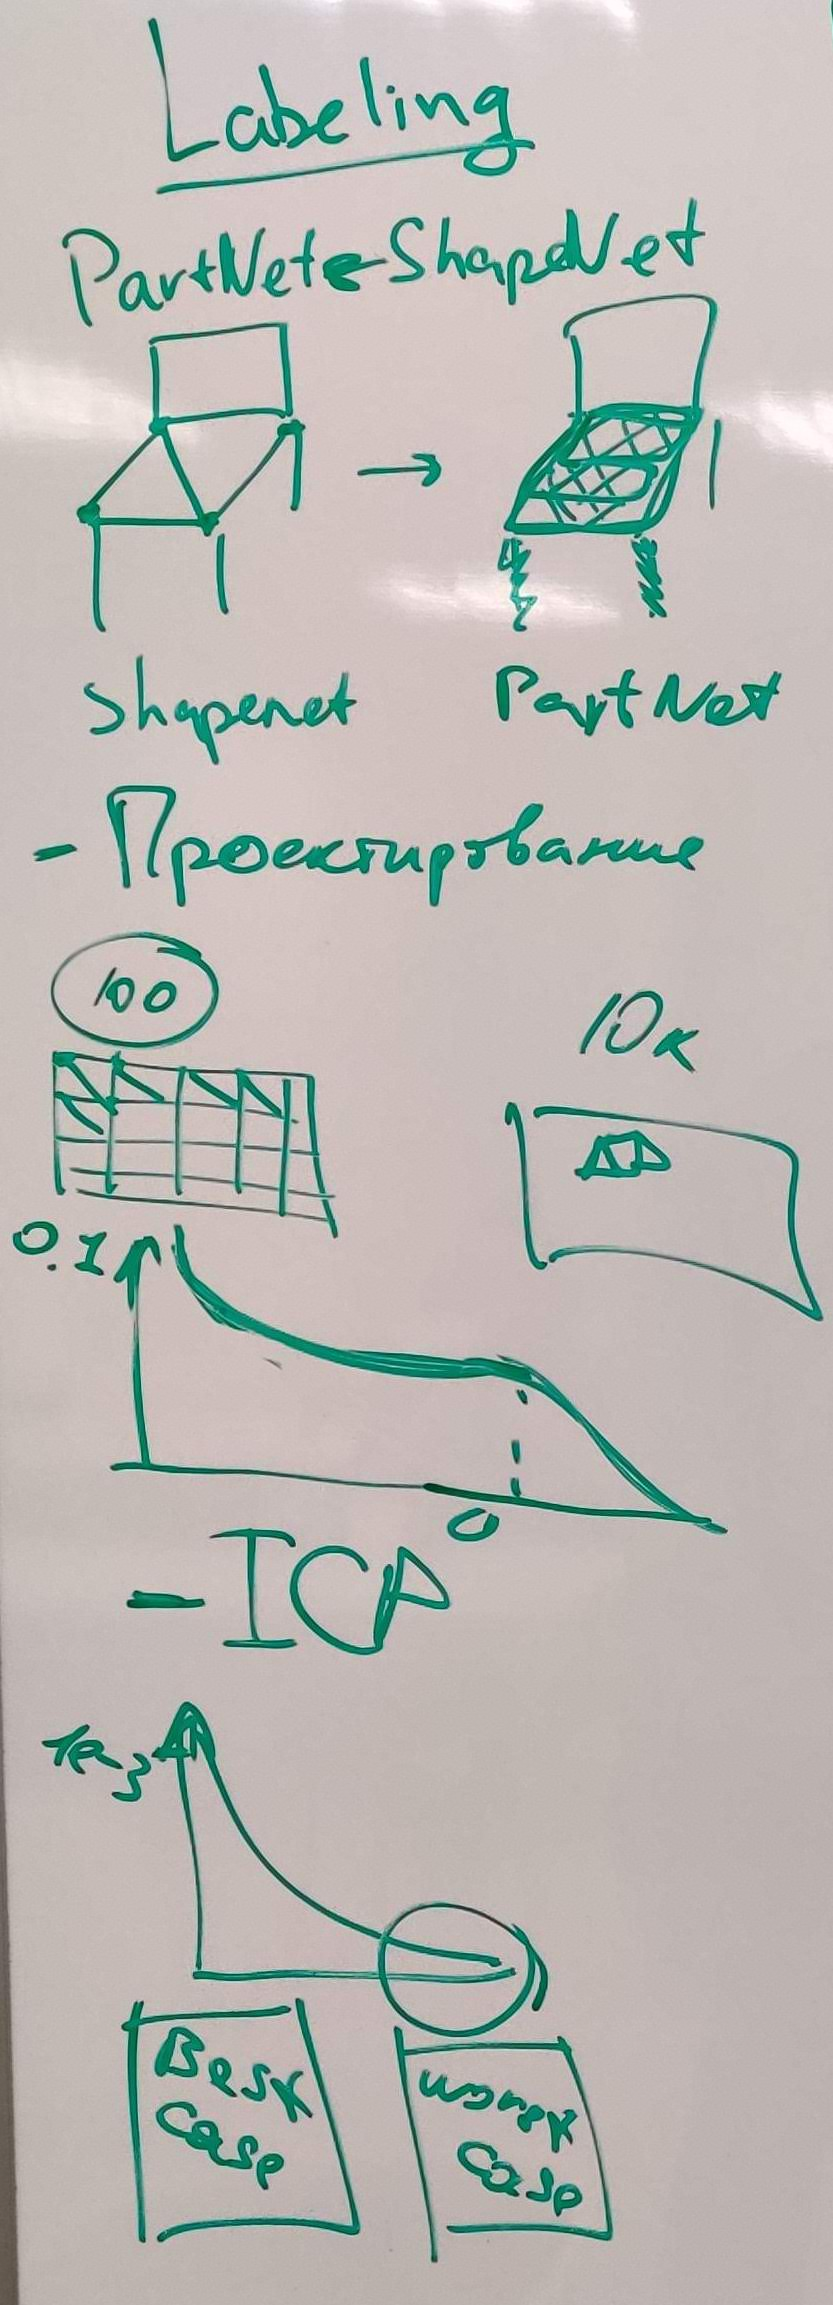
\includegraphics[trim=0 0 0 0, max width=0.25\textwidth]{images/partnet_to_scannet_labeling.jpg}
\caption{partnet to scannet labeling (a,b,c)}
% \end{wrapfigure}
\end{figure}

\begin{figure}[!htb]
\label{fig:scannet_overview}
  \centering
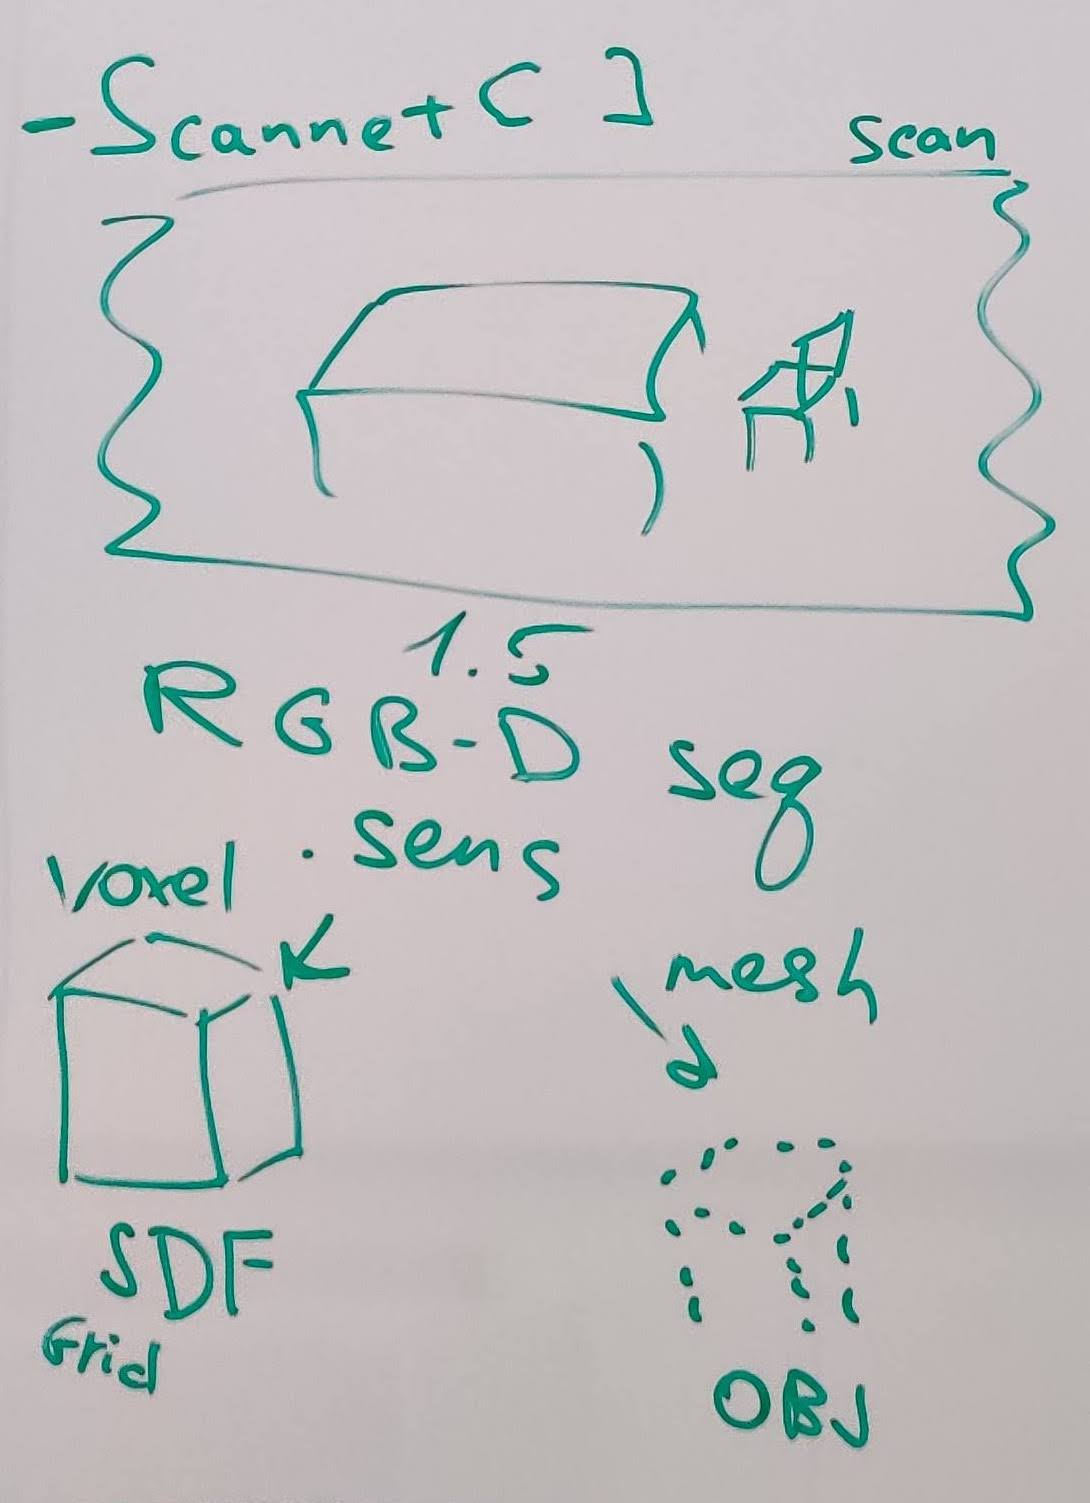
\includegraphics[trim=0 0 0 0, max width=0.5\textwidth]{images/scannet_overview.jpg}
\caption{scannet overview}
\end{figure}

\begin{figure}[!htb]
\label{fig:Scan2Cad_overview}
\centering
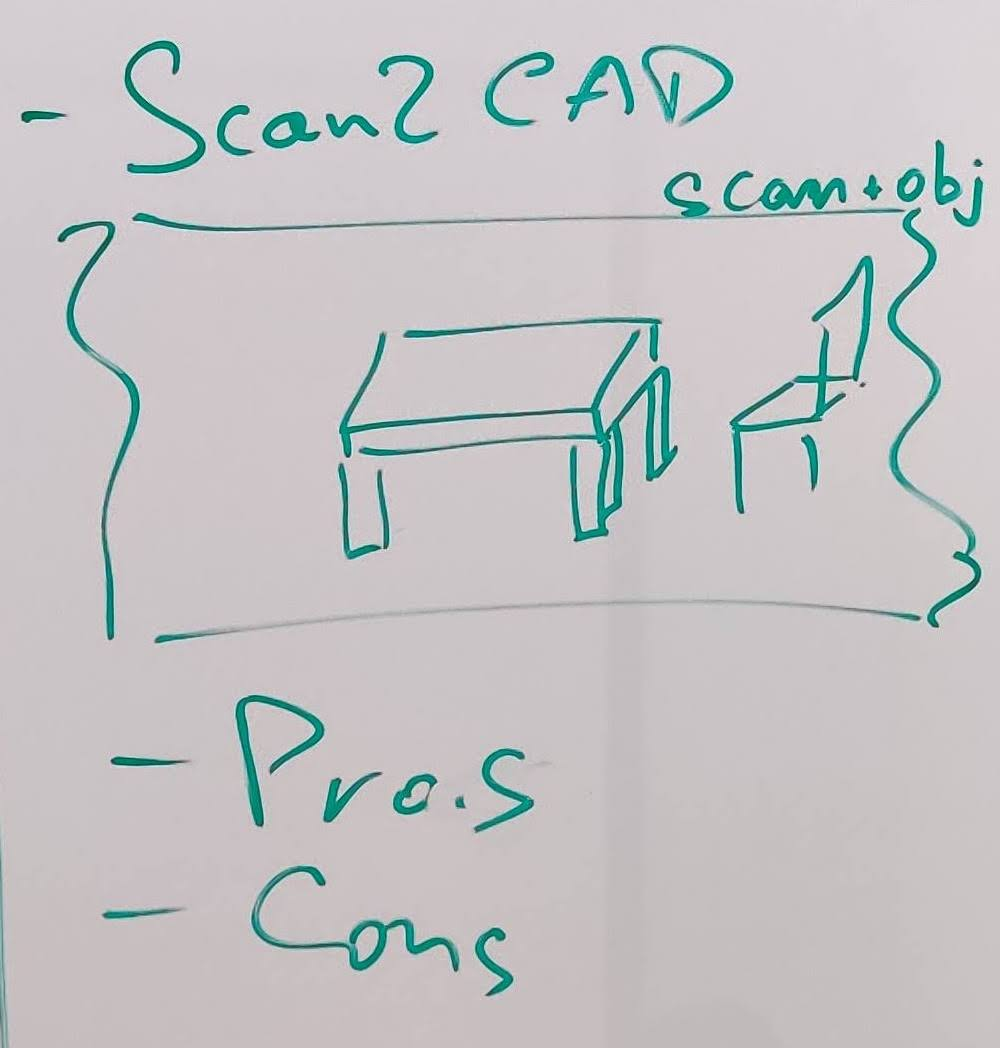
\includegraphics[trim=0 0 0 0, max width=0.5\textwidth]{images/Scan2Cad_overview.jpg}
\caption{Scan2Cad overview}
\end{figure}



\begin{table}[]
\caption{Proportions of ShapeNet semantic classes present in Scan2Cad dataset}
\label{table:scan2part_proportions}
\begin{tabular}{l|l|l}
Class ID & overlap? & class name \\
\hline
04379243 & 99.0\% (822/830) & table \\ \hline
02747177 & 98.9\% (88/89) & ashcan,trash can,garbage can,wastebin,ash bin,ash-bin \\ \hline
03211117 & 97.6\% (161/165) & display,video display \\ \hline
03761084 & 97.3\% (36/37) & microwave,microwave oven \\ \hline
03337140 & 97.1\% (68/70) & file,file cabinet,filing cabinet \\ \hline
03001627 & 96.9\% (632/652) & chair \\ \hline
02871439 & 96.7\% (145/150) & bookshelf \\ \hline
02933112 & 94.8\% (294/310) & cabinet \\ \hline
02818832 & 94.0\% (47/50) & bed \\ \hline
03991062 & 91.7\% (11/12) & pot,flowerpot \\ \hline
03207941 & 85.7\% (12/14) & dishwasher,dish washer,dishwashing machine \\ \hline
03085013 & 81.8\% (9/11) & computer keyboard,keypad \\ \hline
03325088 & 57.1\% (4/7) & faucet,spigot \\ \hline
02876657 & 50.0\% (1/2) & bottle \\ \hline
02808440 & 26.0\% (25/96) & bathtub,bathing tub,bath,tub \\ \hline
02801938 & 9.4\% (3/32) & basket,handbasket \\ \hline
04256520 & 8.1\% (20/247) & sofa,couch,lounge \\ \hline
02946921 & 0.0\% (0/1) & can,tin,tin can \\ \hline
03938244 & 0.0\% (0/5) & pillow \\ \hline
02828884 & 0.0\% (0/28) & bench \\ \hline
04554684 & 0.0\% (0/37) & washer,automatic washer,washing machine \\ \hline
03928116 & 0.0\% (0/25) & piano,pianoforte,forte-piano \\ \hline
03790512 & 0.0\% (0/4) & motorcycle,bike \\ \hline
03691459 & 0.0\% (0/2) & loudspeaker,speaker,speaker unit,loudspeaker system \\ \hline
03467517 & 0.0\% (0/6) & guitar \\ \hline
04330267 & 0.0\% (0/36) & stove \\ \hline
04401088 & 0.0\% (0/1) & telephone,phone,telephone set \\ \hline
04004475 & 0.0\% (0/31) & printer,printing machine \\ \hline
Total:    & 81.2\% (2477/3049) &         \\
\end{tabular}
\end{table}




\subsection{Scene labeling}

\textbf{PartNet -> Shapenet.} The PartNet \cite{mo2019partnet} is a hierarchical instance-level parts dataset of labels for the subset of the ShapeNet database. The PartNet dataset is the only dataset that has a deep hierarchical structure compared to other part annotation datasets, e.g.,  \cite{Yi16}. However, the PartNet dataset does not preserve the original ShapeNet coordinate system in the sense that each object is rotated in an unspecified order. For mapping labels to Scannet scenes, we need to restore the original coordinate system. To find the rotation matrix between coordinate systems, we use the following alignment process for each object: \begin{enumerate}
    \item we sample 20 different rotation angles corresponding to the vertices of the convex regular dodecahedron;
    \item each rotation angle is represented as the initial alignment matrix of the object for alignment;
    \item we perform Point-to-point ICP alignment separately for each initial alignment matrix;
    \item we select the best one out of 20 alignment results where the distance between the original ShapeNet shape and the rotated PartNet shape is minimal.
\end{enumerate}

\textbf{Shapenet -> Scannet (Scan2CAD).} The Scan2CAD \cite{avetisyan2019scan2cad} is a dataset that aligns CAD objects from ShapeNet \cite{chang2015shapenet} database to scenes from Scannet. Using the marching cubes algorithm, we obtained  voxelized versions of scenes from ScanNet dataset with object type labels and mapping of coordinate systems from ScanNet to ShapeNet.  Finally, we  calculate the position of CAD object parts in the scene coordinate system and calculate relative volume in specific voxels thus projecting part labels on the scene. \DZ{unclear what relative volume is needed for here}

Under closer examination, we discovered that most of the parts do not have a unique shape making the task of instance segmentation for parts very hard to solve and not necessary for practical scene segmentation task. \DZ{unclear}
